% Delete the MSc option if you are doing a PhD, or replace it with MPhil
% for a Master of Philosophy thesis
%
% The 12pt option is required by the 2001/02 thesis regulations
% Last update 22nd January 2020: updated department/school/faculty names

% Replace PhD with MSc for MSc theses
% Remove the twoside option for single-sided printing
\documentclass[12pt,PhD,twoside]{muthesis}

%%%%%%%%%%%%%%%%%%%%%%%%%%%%%%%%%%%%%%%%%%%%%%%%%%%%%%%%%%%%%%%%%%%%%%%%%%%%%%%%%%%%%%%%%%%%%%%%%%
% DOCUMENT.
%%%%%%%%%%%%%%%%%%%%%%%%%%%%%%%%%%%%%%%%%%%%%%%%%%%%%%%%%%%%%%%%%%%%%%%%%%%%%%%%%%%%%%%%%%%%%%%%%%
\raggedbottom % Avoid whitespace between paragraphs.
\begin{document}
\title{Title}
\author{Author} % 2019 regulations state middle name(s) should be initials
\department{Mathematics}
\school{Natural Sciences}
\faculty{Science and Engineering}
\def\wordcount{xxxxx} % A word count is required

% Uncomment the line below to suppress the `List of Tables' page (optional)
% \tablespagefalse

% Uncomment the line below to suppress the `List of Figures' page (optional)
%\figurespagefalse

% Uncomment the line below to use a customised Declaration statement
%\def\declaration{All the work in this thesis has been sourced from Google.}

\beforeabstract 

Abstract text here.

\afterabstract

% The next part is optional; however it is a good place to thank your
% supervisor and the people responsible for providing computer support ;-)
\prefacesection{Acknowledgments}

I would like to thank...

% The next line is NOT optional and MUST appear
\afterpreface

% Add the introduction (and then any other chapters...)

\graphicspath{{intro/figs/}}

\chapter{Introduction}
\chaptermark{Introduction} 
\label{intro}

This is the introduction. Figure \ref{intro.fig} shows how figures are presented. Table \ref{intro.tb} does likewise for tables and Algorithm \ref{intro.alg} for algorithms. This is a reference to a book \cite{and99} and this to an article \cite{don90}.

\section{Section}
\sectionmark{Section}
\label{intro.section}

This is a new section.

      \begin{figure}
	\centering	
	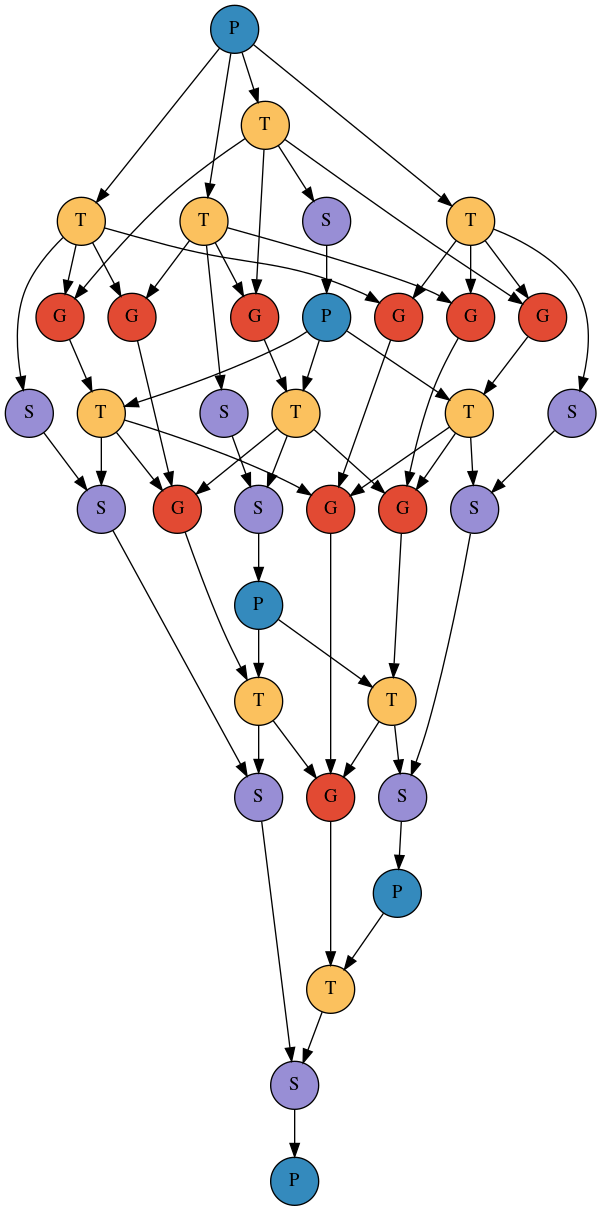
\includegraphics[scale=0.3]{cholesky35.png}
	\caption{This is an example figure.}	
	\label{intro.fig}
      \end{figure}

      \subsection{Subsection}
      \label{intro.section.subsection}

      This is a subsection.

              \begin{table}
        \centering
        \caption{This is an example table.} 	
        \begin{tabular}{c c c c c}
         \toprule
         Tile size & {\tt GEMM} & {\tt POTRF} & {\tt SYRK} & {\tt TRSM} \\
         \cmidrule{1-5}
         $128$ & $8.0$ & $1.7$ & $2.3$ & $1.7$ \\
         $1024$ & $92.7$ & $13.7$ & $55.8$ & $24.2$ \\             
        \bottomrule
        \end{tabular}   
        \label{intro.tb}
        \end{table}

\begin{algorithm}	
	
	\For{$i = 1, \dots, N$}
	{
		$A_{ii} = {\tt POTRF}(A_{ii})$
		
		\For{$j = i + 1, \dots, N - 1$}{$A_{ji} = {\tt TRSM}(A_{ii}, A_{ji})$}
		
		\For{$k = i + 1, \dots, N - 1$}
		{
			$A_{kk} = {\tt SYRK}(A_{ki}, A_{kk})$
			
			\For{$j = k + 1, \dots, N - 1$}{$A_{jk} = {\tt GEMM}(A_{ji}, A_{ki}, A_{jk})$}
		}		
	}	
	
	\caption{This is an example algorithm.}
	\label{intro.alg}
      \end{algorithm} 



%%% Local Variables:
%%% mode: latex
%%% TeX-master: "<none>"
%%% End:


% Bibliography.
\printbibliography[heading=bibintoc, title={Bibliography}]

\end{document}


%%% Local Variables:
%%% mode: latex
%%% TeX-master: t
%%% End:
